\chapter{Desenvolvimento}\label{cap_desenv}

Para o desenvolvimento das atividades inicialmente foi escolhido duas base de dados. As bases foram encontradas no site http://cs.uef.fi/sipu/datasets/ onde possuem datasets próprios para a tarefa de clustering, os dataset não possuem informações de que se referem cada atributo ou cada instancia.

\section{Pré-processamento e Visualização}
Para realizar o pré-processamento foi necessário validar se os dados não possuiam números vazios ou algum tipo de valor que foge do esperado.


\section{Validação dos dados}
Foi validado que os dataset não possuem nenhum valor nulo ou valores diferentes de inteiro maior do que zero.

\section{Análise dos dados}
Com os valores todos normalizados podemos ver a correlação entre os atributos, que possuem alta relação em alguns casos. \ref{fig:correlacao}

\begin{figure}[h]
	\centering
	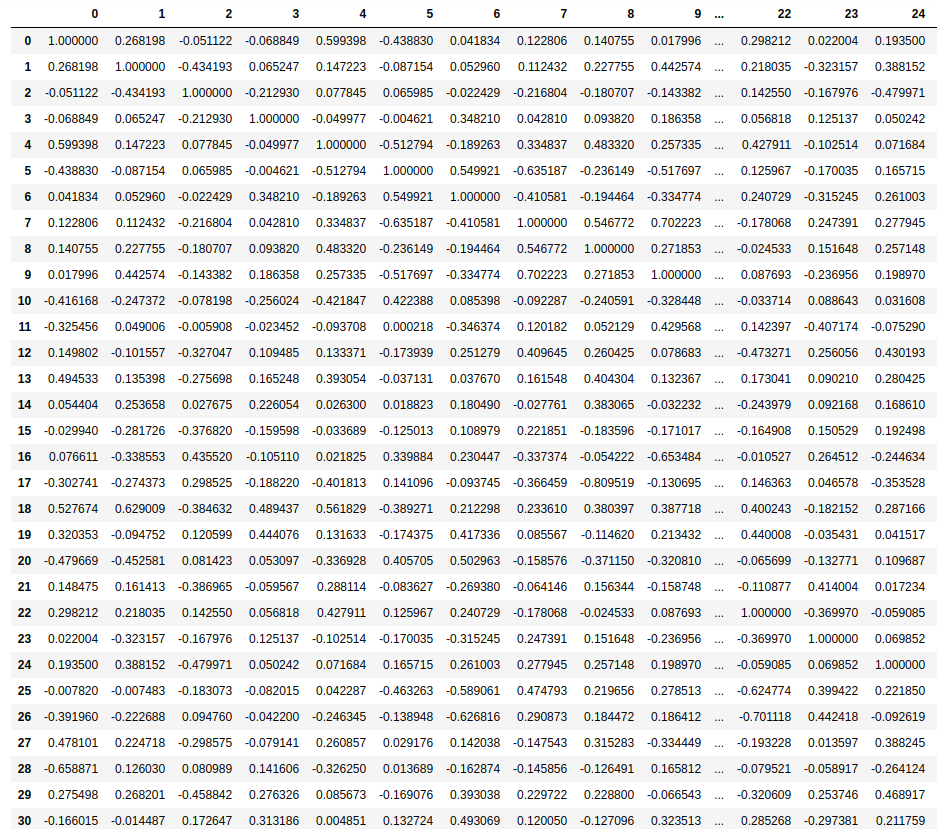
\includegraphics[width=0.7\linewidth]{images/corr}
	\caption{Correlação entre os dados.}
	Fonte: pessoal.
	\label{fig:correlacao}
\end{figure}

Após a visualazação dos dados foi gerado o bloxpot \ref{fig:bloxpot} para ver como está a distribuição dos dados onde é possível ver que poucos atributos possuem outliers e os dados possuem certa distribuição padrão, e também os valores de media, moda e mediana para cada atributo.\ref{fig:describe}

\begin{figure}[h]
	\centering
	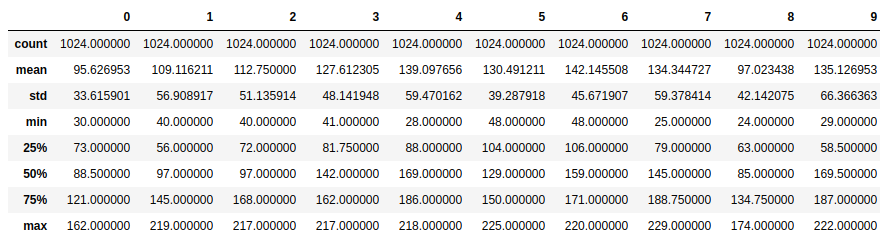
\includegraphics[width=0.7\linewidth]{images/describe}
	\caption{Distribuição dos dados.}
	Fonte: pessoal.
	\label{fig:describe}
\end{figure}

\begin{figure}[h]
	\centering
	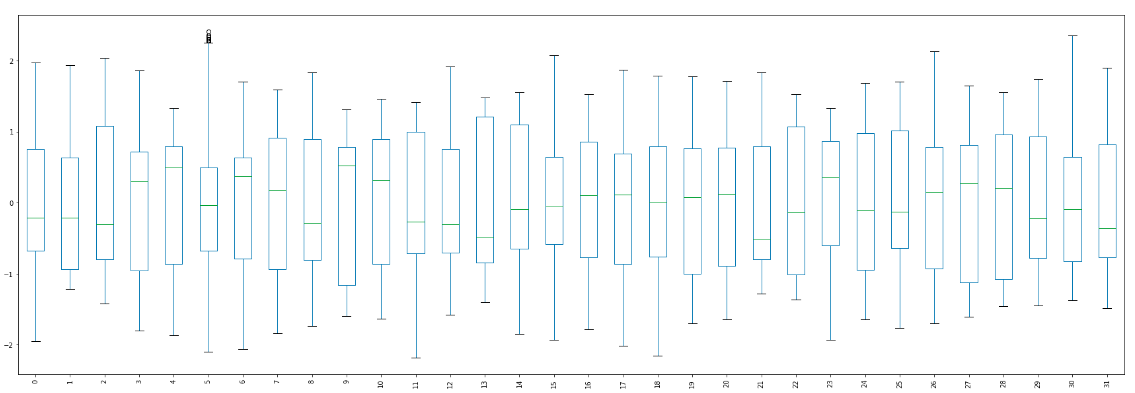
\includegraphics[width=0.7\linewidth]{images/bloxpot}
	\caption{Bloxpot exibindo outliers.}
	Fonte: pessoal.
	\label{fig:bloxpot}
\end{figure}


\section{Escalonamento}
Para aplicar os algoritmos de clustering, é necessário escalonar os dados, normalizando eles em uma faixa de -1 a 1, onde os dados irão manter a mesma proporção e similaridades.


\section{Seleção de atributos}

Após executar os três algoritmos de classificação com o dataset em questão, foi realizado um processo de seleção de atributos para realizar novamente a execução destes mesmos algoritmos.

O dataset possuia 32 atributos numericos, para realizar a selação foi utilizado um algoritmo que utiliza um parametro k como score para selecionar os melhores atributos.

Neste dataset o algoritmo selecionou apenas 4 atributos
